\documentclass{article}
\usepackage{xcolor}
\usepackage{tikz}
\usetikzlibrary{cd}
\usetikzlibrary{arrows}
\usepackage{amssymb,amsmath,amsthm,mathtools,slashed,bm}

\begin{document}

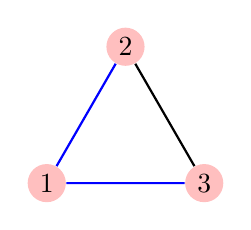
\begin{tikzpicture}[shorten >=1pt,->]
    \tikzstyle{vertex}=[circle,fill=red!25,minimum size=12pt,inner sep=2pt]
    \node[vertex] (G_1) at (0,0) {1};
    \node[vertex] (G_2) at (1,1.732)   {2};
    \node[vertex] (G_3) at (2,0)  {3};
    \draw[color=blue,thick] (G_2) -- (G_1) -- (G_3) -- cycle;
    \draw[thick] (G_2) -- (G_3) -- cycle;
    \end{tikzpicture}

\end{document}